\section{Testset}
\label{sec:testset}
Bij de testset is ervoor gekozen om een oppervlakkige tekening te maken van België in een aangepaste schaal. Deze keuze is gemaakt vanwegen meerdere redenen. Om te beginnen laat deze aangepaste schaal zeer makkelijk toe om (als mens) vlakken te beschrijven. Aangezien dit een technisch en bovendien vooruitstrevend onderwerp is, is het handig om terug te keren naar een bekender terein. Daarom is de bekendheid van deze \textit{use case} meteen de tweede reden van deze keuze. Een derde reden is dat deze dataset eerder klein is, waardoor mogelijke fouten of onlogische oplossingen hierbij nogmaals getest worden. Ten slotte is dit ook de perfecte dataset voor het geven van demonstraties omdat deze set herkenbaar is voor het publiek. Een visualisatie van deze dataset is te zien in \figureref{fig:demoset}. De effectieve dataset is dan weer te vinden op GitHub Gist\footnote{https://gist.github.com/dreeki/e48bbe533a4b1191045b3652ff2c9c81}. Deze dataset is bovendien opgesplitst in vijf verschillende bestanden (namelijk: ``land'', ``gewest'', ``provincie'', ``weg'' en ``stad'') zodat deze dataset bruikbaar is voor het verifiëren dat gefedereerd queryen nog steeds mogelijk is. Het geheel van deze testing wordt uitgevoerd in de testomgeving die besproken werd in \sectionref{sec:testomgeving}. Hierbij zorgt de \textit{execution log} ervoor dat alles duidelijk is hoe het geheel in zijn werk gaat.

\begin{figure}
    \centering
    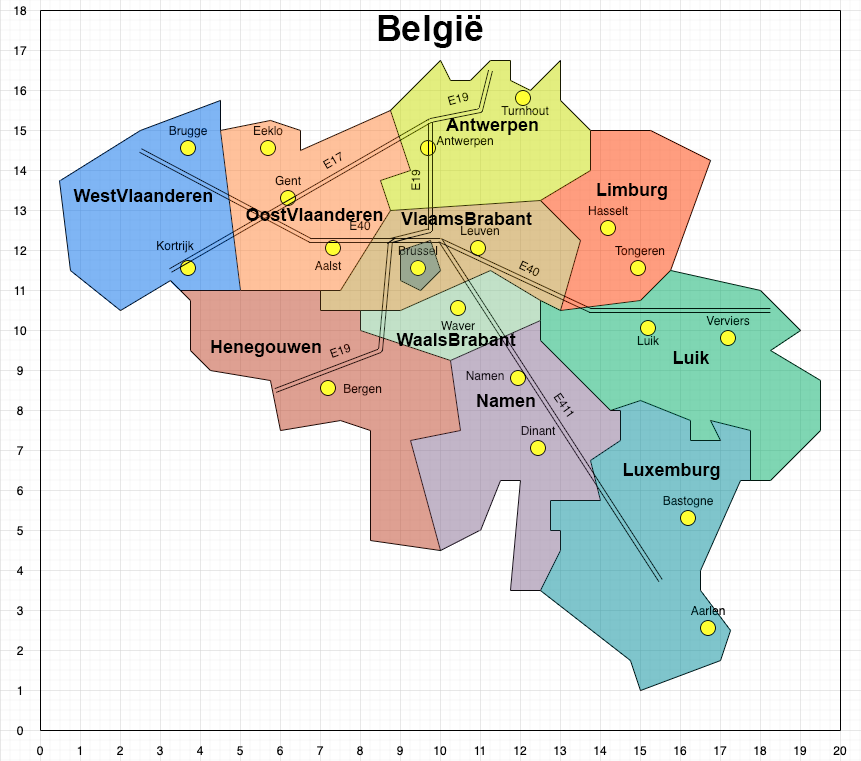
\includegraphics[width=\linewidth]{images/geosparql_demo.png}
    \caption{Testset voor het testen van de verschillende bronnen.}
    \label{fig:demoset}
\end{figure}


\subsection{queries}
Voor de uitvoering van de tests zijn verschillende queries opgesteld om mee te testen. In de testomgeving zelf kunnen hierbij vervolgens de bronnen aangepast worden naar de te testen bronnen. Het is echter wel nog op te merken dat de ontologieën bij de testomgeving reeds in code aangegeven werden. Bij gevolg worden deze niet opnieuw mee opgenomen in de geschreven query, maar in de achtergrond worden deze dus wel nog gebruikt.
\todo{my:hasExactGeometry aanpassen en op gist aanpassen!}


\subsubsection{Query 1}
De eerste \textit{query} zoekt naar alle provincies die binnen Vlaanderen liggen. Om dit te kunnen doen zal de \textit{query engine} eerst de vorm van Vlaanderen zelf opzoeken. Daarna zal hij de vorm van alle provincies zoeken zodat hij met de ``sfContains'' functie van GeoSPARQL uiteindelijk kan filteren. Deze query is te zien in \listingref{listing:find_provinces_flanders}.

\begin{listing}[ht]
    \begin{minted}{sparql}
        SELECT ?f
        WHERE {
            gewest:Vlaanderen my:hasExactGeometry ?aGeom .
            ?aGeom geo:asWKT ?aWKT .
            ?f a my:Provincie .
            ?f my:hasExactGeometry ?fGeom .
            ?fGeom geo:asWKT ?fWKT .
            FILTER (geof:sfContains(?aWKT, ?fWKT))
        }
    \end{minted}
    \caption{Find all the provinces in Flanders.}
    \label{listing:find_provinces_flanders}
\end{listing}


\subsubsection{Query 2}
De tweede \textit{query} is zeer gelijkaardig aan de eerste, maar hier is één groot verschil. Deze \textit{query} zoekt naar alles dat binnen Vlaanderen ligt. Aangezien ``sfContains'' functie stelt dat een geospatiaal identieke vorm steeds binnen de andere ligt, zou deze query Vlaanderen zelf ook als een oplossing zien. Aangezien dit niet het verwachte resultaat is, wordt gebruik gemaakt van de negatie van de ``sameterm'' functie van SPARQL. Dit wijst er nogmaals op dat een werkende implementatie van SPARQL een vereiste is voor het maken van een GeoSPARQL implementatie. Deze query is te zien in \listingref{listing:find_everything_flanders}.

\begin{listing}[ht]
    \begin{minted}{sparql}
        SELECT ?f
        WHERE {
            gewest:Vlaanderen my:hasExactGeometry ?aGeom .
            ?aGeom geo:asWKT ?aWKT .
            ?f my:hasExactGeometry ?fGeom .
            ?fGeom geo:asWKT ?fWKT .
            FILTER (geof:sfContains(?aWKT, ?fWKT) && !sameterm(?aWKT, ?fWKT))
        }
    \end{minted}
    \caption{Find everything that's geospatially inside Flanders.}
    \label{listing:find_everything_flanders}
\end{listing}


\subsubsection{Query 3}
De derde query gaat dan weer over het vinden van de wegen en provincies die binnen België liggen. Deze query toont nogmaals aan hoe gelijkaardig SQL en SPARQL zijn. Deze query is te zien in \listingref{listing:find_provinces_roads_belgium}.

\begin{listing}[ht]
    \begin{minted}{sparql}
        SELECT ?f
        WHERE {
            land:België my:hasExactGeometry ?aGeom .
            ?aGeom geo:asWKT ?aWKT .
            {
                ?f a my:Provincie .
            }
                UNION
            {
                ?f a my:Weg .
            }
            ?f my:hasExactGeometry ?fGeom .
            ?fGeom geo:asWKT ?fWKT .
            FILTER (geof:sfContains(?aWKT, ?fWKT))
        }
    \end{minted}
    \caption{Find all the provinces and roads in Belgium.}
    \label{listing:find_provinces_roads_belgium}
\end{listing}


\subsubsection{Query 4}
Bij de vierde query worden alle wegen die door Oost-Vlaanderen gaan opgezocht. Dit zou bijvoorbeeld handig kunnen zijn wanneer iemand de snelwegen wil vinden die makkelijk bereikbaar zijn vanuit Oost-Vlaanderen. Hierbij wordt de functie ``sfIntersects'' van GeoSPARQL gebruikt. Deze query is te zien in \listingref{listing:find_roads_passing_east_flanders}.

\begin{listing}[ht]
    \begin{minted}{sparql}
        SELECT ?f
        WHERE {
            prov:OostVlaanderen my:hasExactGeometry ?aGeom .
            ?aGeom geo:asWKT ?aWKT .
            ?f a my:Weg .
            ?f my:hasExactGeometry ?fGeom .
            ?fGeom geo:asWKT ?fWKT .
            FILTER (geof:sfIntersects(?aWKT, ?fWKT))
        }
    \end{minted}
    \caption{Find all the roads that pass through East-Flanders.}
    \label{listing:find_roads_passing_east_flanders}
\end{listing}


\subsubsection{Query 5}
De vijfde query toont aan dat het mogelijk is om manueel een vorm te voorzien om op te filteren. Deze vorm staat (bij de aangepaste schaal) voor de \textit{bounding box} van Vlaams-Brabant en Waals-Brabant. Deze query zal alles weergeven dat zich binnen deze vorm bevindt. Voor de verandering wordt hier de ``sfWithin'' functie van GeoSPARQL gebruikt, maar dit zou evengoed mogelijk zijn met de ``sfContains'' functie. Deze query is te zien in \listingref{listing:find_everything_bounding_box}.

\begin{listing}[ht]
    \begin{minted}{sparql}
        SELECT ?f
        WHERE {
            ?f my:hasExactGeometry ?fGeom .
            ?fGeom geo:asWKT ?fWKT .
            FILTER (geof:sfWithin(?fWKT, '''Polygon((7 9.25, 13.5 9.25, 13.5 13.25, 
            7 13.25, 7 9.25))'''^^geo:wktLiteral))
        }
    \end{minted}
    \caption{Find everything inside the bounding box of Brabant.}
    \label{listing:find_everything_bounding_box}
\end{listing}




\todo{misschien nog extra queries}